% \chapter{Search spaces}


Before going further with our quest for efficient RL. Let's try to understand
some properties of our setting, tabular MDPs.

\newpage

\section{The value function polytope}

The Value Function Polytope \cite{Dadashi2018} provides intuition
about the structure of a MDP and the dynamics and complexity of solvers.
Let's take a look: consider a two state, two action MDP.

\begin{figure}[hb!]
\centering
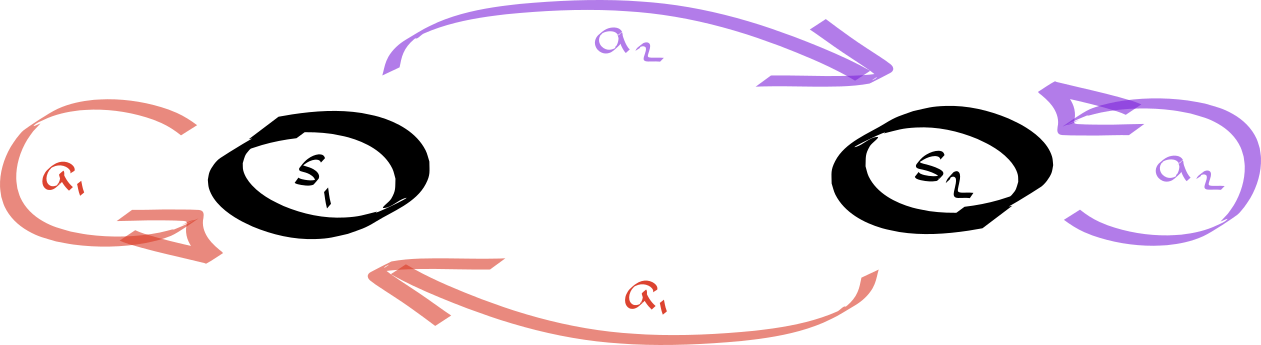
\includegraphics[width=1\textwidth,height=0.25\textheight]{../../pictures/drawings/2-state-automata.png}
\caption{The simplest possible MDP has two states and two actions. (Any simpler setting is entirely uninteresting. A single state means actions do nothing.
A single action means all policies are the same.).}
\end{figure}

The space of possible policies is a 2D surface in a 4D space. For each state, we
can pick \texttt{action1} or \texttt{action2}, with some probability, $p$. For more intuition
about this policy space see \ref{high-D-policies}.
And for a method of visualising higher dimensional policies, see \ref{graph-vis}.

\begin{align}
\pi &=
\begin{bmatrix}
  p(a=a_1|s=s_1) & p(a=a_2|s=s_1) \\
  p(a=a_1|s=s_2) & p(a=a_2|s=s_2)\\
\end{bmatrix} \\
&=
\begin{bmatrix}
p(a=a_1|s=s_1) & 1-p(a=a_1|s=s_1) \\
p(a=a_1|s=s_2) & 1-p(a=a_1|s=s_2)\\
\end{bmatrix}
\end{align}

Since the policies are a 2D space, we can visualise them. This square of all possible policies is not particularly interesting.

Rather, we can evaluate (calculate the expected return) each policy (using the \eqref{eq:value-functional}).
Since there are two states, the evaluation returns a 2D vector of values, one value for each state.
Therefore, we can visualise the value of each policy.
\begin{figure}[!hb]
\centering
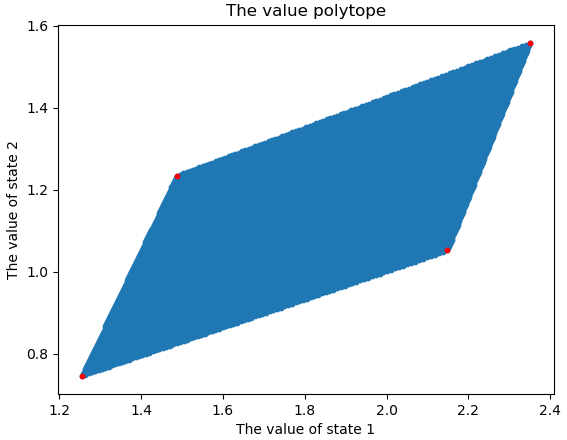
\includegraphics[width=1\textwidth,height=0.5\textheight]{../../pictures/figures/value-polytope.png}
\caption{For every policy, we can plot a dot that represents the value of that policy.
The red dots are deterministic policies.}
\end{figure}

Dadashi et al. \cite{Dadashi2018} explored a few properties of the polytope.
Specifically they focused on its geometry and dynamics.

\subsubsection{Geometry of the polytope}\label{geom-polytope}

Dadashi et al. remark; the polytope gives a clear illustration of the following classic results regarding MDPs \cite{Bertsekas1996}.

\begin{enumerate}
\tightlist
  \item (Dominance of $V^*$) The optimal value function $V^*$ is the unique dominating vertex of $V$;
  \item (Monotonicity) The edges of V are oriented with the positive orthant;
  \item (Continuity) The space V is connected.
\end{enumerate}

Let's try to understand these.

\paragraph{Dominance} By the definition of the optimal policy, $\forall s: V^{\pi^{*}}(s)\ge V^{\pi}(s)$.
Imagine there is some other policy, $\pi'$ and state $s'$, such that $V^{\pi^{*}}(s')\le V^{\pi'}(s')$. This is a contradiction.
Thus, the optimal value function must have the largest value in all states, meaning it will be the 'dominating' vertex.

\paragraph{Monotonicity} If $V(s_2)$ increases then $V(s_1)$ must either increase or stay the same.
This can be seen in the last equation below;

\begin{align*}
V(s_1) &= \mathop{\mathbb E}_{a \sim\pi(\cdot|s_1)} r(s, a) + \gamma \mathop{\mathbb E}_{s'\sim \sum_a \tau(\cdot|s, a)\pi(\cdot|s)} V(s')\\
&= \sum_a \pi(a|s_1)r(s, a) + \gamma \sum_{s'}\sum_a \tau(s'|s_1, a)\pi(a|s) V(s') \\
&= \sum_a \pi(a|s_1)r(s, a) + \gamma \sum_a \tau(s_1|s_1, a)\pi(a|s) V(s_1) + \gamma\sum_a \tau(s_2|s_1, a)\pi(a|s) V(s_2)
\end{align*}

If $\sum_a \tau(s_2|s_1, a)\pi(a|s) = 0$ (i.e. $s_1$ and $s_2$ are not connected)
then $V(s_1)$ stays the same, yielding a constant vertical line on the polytope.
If $\sum_a \tau(s_2|s_1, a)\pi(a|s) > 0$ (i.e. there is some change of transitioning from $s_1$ to $s_2$)
then $V(s_1)$ increases with $V(s_2)$, yielding a 'positive orthant'.
$\sum_a \tau(s_2|s_1, a)\pi(a|s) < 0$ is not possible.

\paragraph{Continuity} The policy space is connected by definition, and the value function is a continuous function.
Therefore the value space, the polytope, is connected.

\subsubsection{Dynamics on the polytope}

Furthermore, Dadashi et al. \cite{Dadashi2018} were interested in three aspects of different algorithms’ learning dynamics;

\begin{itemize}
\tightlist
  \item the path taken through the value polytope,
  \item the speed at which they traverse the polytope,
  \item any accumulation points that occur along this path.
\end{itemize}

% Why do they care?
% How quickly do these learners traverse the polytope? Do algorithms take the shortest path? Where are the accumulation points?

They consider value iteration, policy iteration, policy gradients, entropy regularized policy gradients,
natural policy gradients and the cross entropy method.

Their results are intriguing. They show that different RL algorithms traverse the polytope in vastly different ways.
Some are not even constrained to the polytope. This raises the question;

\begin{displayquote}
  \textsl{How does a search algorithm interact with its search space to yield efficient search?}
\end{displayquote}

\begin{center}\rule{0.5\linewidth}{\linethickness}\end{center}

In \ref{polytope-extras} you can find further exploration of other properties of
the value polytope, such as; the density of policies, and the effect of the discount
rate.

\newpage
\section{Search spaces for MDPs}\label{search-spaces-mdps}

We want to efficiently find the optimal policy for a given MDP. But where and how should we
search for this policy? We could search within;

\begin{itemize}
\tightlist
  \item the set of potentially optimal policies, the $|A|^{|S|}$ discrete policies,
  \item the set of all possible policies $\pi \in \mathbb R^{|S| \times |A|}: \int_a \pi(a|s) = 1 \forall s $
  \item the set of possible state-action value functions, $\mathbb R^{|S|\times|S|}$,
  (which we could then use to construct the optimal policy),
  \item Or maybe some other space?
\end{itemize}

\begin{displayquote}
  \textsl{Which space is best? Which space allows us to find the optimal policy in the 'cheapest' manner?}
\end{displayquote}

Naively, we often think smaller search spaces are better. We would rather
search for our keys in a few rooms, rather than many. But added
structure (for example, ordering) can be exploited to yield faster
search, even when there are infinitely more states to search. For example,
we might be able to order the rooms based on how recently we visited them.
This should help us retrace our steps and find our keys, rather than arbitrarily
picking rooms to search.

\subsection{Policy search}

We can search through policies. In my opinion, this is the most 'natural' type of search for RL.
As, after all, we are searching for the optimal \underline{policy}.

Searching through the space of policies supports a couple of modes of travel:
policy iteration and policy gradients.

\subsubsection{Policy iteration}

In policy iteration (PI), we search for the optimal policy by evaluating our current
policy and then acting greedily. In our tabular setting, policy iteration can be written as:

\begin{algorithm}[H]
\caption{Policy iteration}
\begin{algorithmic}[1]

\Procedure{PI}{$\tau, r, \gamma$}
    \State $t=0$
    \State $\pi_t \sim \mathcal N$  \Comment{Initialise randomly}
    \While{not converged}
      \State $V_t = (I-\gamma \tau_{\pi_t})^{-1} r_{\pi_t}$ \Comment{Evaluate policy}
      \State $Q_t =  r + \gamma \tau\cdot_{s'} V_t$ \Comment{Bellman operator}
      \State $\pi_t = \text{greedy}(Q_t) $ \Comment{Greedy update}
      \State $t = t + 1$
    \EndWhile
    \State \algorithmicreturn{ $\pi_t$}
\EndProcedure

\end{algorithmic}
\end{algorithm}

The greedy operator picks the actions that give the highest state-action return,
and sets their probability to be $1$.
$\text{greedy}(Q) = \text{onehot}(\text{argmax}_a Q[s, a], |A|)$.

This iteration converges because the state-action values capture counterfactuals, $Q^{\pi}(s, a)$.
\textit{What would the return be if I took an action, $a$, not necessarily chosen by
the current policy, then I followed the current policy.}
If there exists an action that achieves higher return than the current policy's choice of action,
then (because of the greedy step) the PI updates to pick that action.

\begin{figure}[h!]
\centering
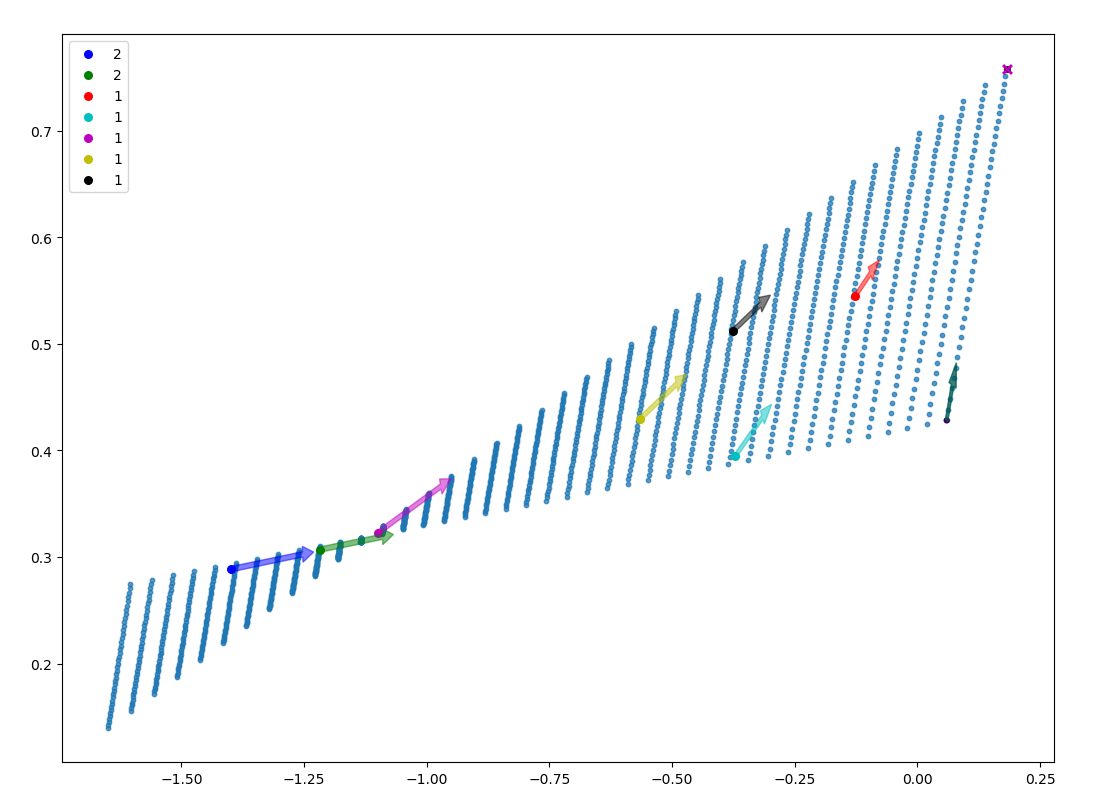
\includegraphics[width=0.7\textwidth,height=0.35\textheight]{../../pictures/figures/pi-polytope.png}
\caption{The optimal policy is shown by the cross.
Each color shows PI applied to a different policy initialisation.
The labels denote the number of iterations to reach convergence.
The arrows point from the current to the next policy. As we can see,
PI jumps between the deterministic policies (the vertices of our polytope).
This is because of the greedy update step.}
\end{figure}

\newpage
\subsubsection{Policy gradients}

Policy gradients (PG) are closely related to the deep learning / end-to-end paradigm.
\textit{Simply write down what you want (the loss function),
estimate its derivative and apply gradient descent.} In our case, the loss function
is the state value function. We can estimate the derivative
by differentiating the \ref{eq:value-functional} with respect to the policy.

To ensure the optimisation problem is constrained properly (that the policy returns a distribution over actions),
we pick $\theta$ as our parameters and construct the policy using $\pi = \sigma(\theta)$, where $\sigma$ is the softmax function.

\begin{algorithm}[H]
\caption{Policy gradients}
\begin{algorithmic}[1]

\Procedure{PG}{$\tau, r, \gamma, \eta$}
  \State $t=0$
  \State $\theta_t \sim \mathcal N$ \Comment{Initialise randomly}
  \While{not converged}
    \State $\theta_{t+1} = \pi_t + \eta \nabla_{\theta} V(\sigma(\theta_t))$ \Comment{Gradient update}
    \State t += 1
  \EndWhile
  \State \algorithmicreturn{ $\sigma(\theta_t)$}
\EndProcedure

\end{algorithmic}
\end{algorithm}

To mitigate stability / convergence issues, it is common to add weak regularisation,
which maximises the entropy of the policy. This forces policies away
from the edges of the polytope, where gradients are not defined.

\begin{figure}[h!]
\centering
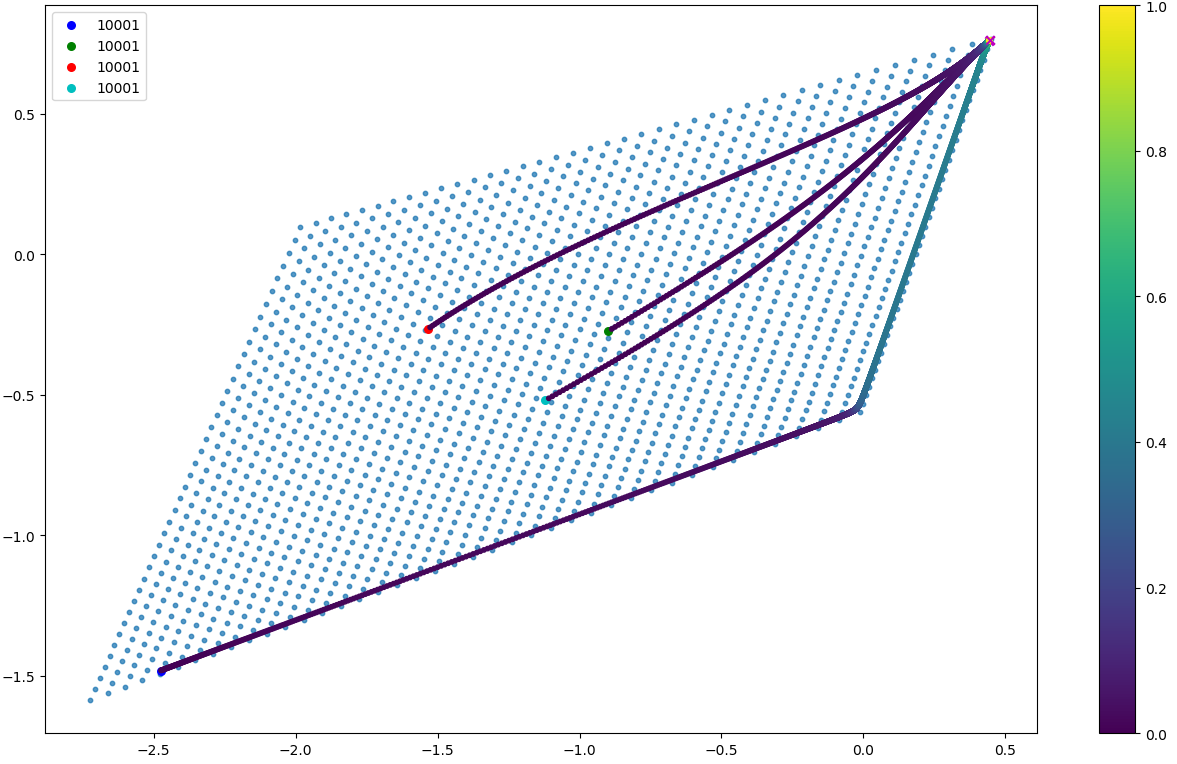
\includegraphics[width=0.7\textwidth,height=0.35\textheight]{../../pictures/figures/pg-polytope.png}
\caption{
Examples of policy gradients: observe that most of the trajectories are purple,
indicating that the majority of progress is made in the first 20\% of training.
They converge very slowly once close to the optimal policy.}
\end{figure}

% Want to include upper / lower bounds!?
% {\color{red}??? Converges at a rate of $\frac{1}{t}$. As can be seen by ...}
% \cite{Agarwal2019a}.

\newpage
\subsection{Value search}

Alternatively, we can search through possible state values, then infer the policy that achieves that value.
But how can we ensure that our search will converge to a value that corresponds to a realisable policy? We can use Bellman's
optimality operator to constrain the search.

(For similar reasons to why policy iteration converges) The greedy step using the
state-action values will find actions with higher value.

\begin{algorithm}[H]
\caption{Value iteration}
\begin{algorithmic}[1]

\Procedure{VI}{$\tau, r, \gamma, \eta$}
  \State t = 0
  \State $V_t = \mathcal N$ \Comment{Initialise randomly}
  \While{not converged}
    \State $\hat V = \text{max}_a T(Q)$  \Comment{Bellman optimality}
    \State $V_{t+1} = V_t + \eta \hat V - V_t$ \Comment{Average temporal difference}
    \State $t += 1$
  \EndWhile
  \State $\pi = \mathop{\text{argmax}}_{\pi} r_{\pi} + \gamma \tau_{\pi}V_t$
  \State \algorithmicreturn{ $\pi$}
\EndProcedure

\end{algorithmic}
\end{algorithm}

% {\color{red}important. Also, why does it go outside?!?}


% Want to include upper / lower bounds!? On complexity. Sample / computational!?
% {\color{red}(need to explain? why does stationarity mean optimality...?!)}
% Intuition about why it converges!? Contraction. Banach fixed-point theorem.

\begin{figure}[h!]
\centering
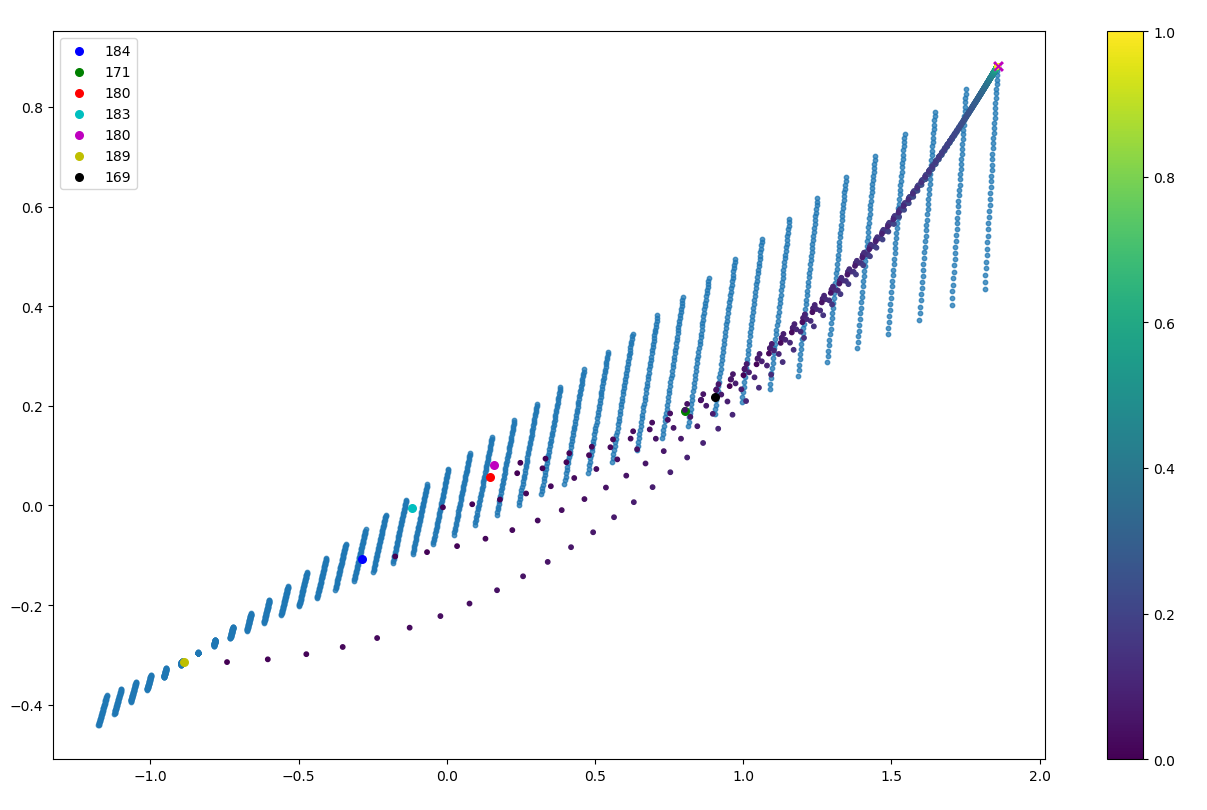
\includegraphics[width=0.7\textwidth,height=0.35\textheight]{../../pictures/figures/vi-polytope.png}
\caption{Observe that the value iterations are not constrained to map to a realisable policy
(they can go out side of the polytope), but they do converge to a realisable policy,
the optimal one.}
\end{figure}


\newpage
\begin{center}\rule{0.5\linewidth}{\linethickness}\end{center}

Thus, there are different classes of search space: each imbued with special
structure from the Bellman equation or expected return. Each with different types of search they
support.

\begin{displayquote}
\textit{Which spaces support efficient search for the optimal policy? Can we characterise the properties of each space?}
\end{displayquote}

For further exploration of search spaces (their iteration complexity and dynamics) see appendix \ref{ss-extras}.
